\documentclass[9pt]{pnas-new}
% Use the lineno option to display guide line numbers if required.
% Note that the use of elements such as single-column equations
% may affect the guide line number alignment. 

%\RequirePackage[english,slovene]{babel} % when writing in slovene
\RequirePackage[slovene,english]{babel} % when writing in english
\usepackage{subcaption}

\usepackage[demo]{graphicx}
\templatetype{pnasresearcharticle} % Choose template 
% {pnasresearcharticle} = Template for a two-column research article
% {pnasmathematics} = Template for a one-column mathematics article
% {pnasinvited} = Template for a PNAS invited submission

%\selectlanguage{slovene}
%\etal{in sod.} % comment out when writing in english
%\renewcommand{\Authands}{ in } % comment out when writing in english
%\renewcommand{\Authand}{ in } % comment out when writing in english

\newcommand{\set}[1]{\ensuremath{\mathbf{#1}}}
\renewcommand{\vec}[1]{\ensuremath{\mathbf{#1}}}
\newcommand{\uvec}[1]{\ensuremath{\hat{\vec{#1}}}}
\newcommand{\const}[1]{{\ensuremath{\kappa_\mathrm{#1}}}} 

\newcommand{\num}[1]{#1}

\graphicspath{{./fig/}}

\title{Emotion contagion model for dynamical crowd path planning}

% Use letters for affiliations, numbers to show equal authorship (if applicable) and to indicate the corresponding author
\author{Andrej Sušnik}
\author{Timotej Zgonik}
\author{Ema Leila Grošelj}

\affil{Collective behaviour course research seminar report} 

% Introduction, Methods, Results and Discussion

% Please give the surname of the lead author for the running footer
\leadauthor{Sušnik} 

\selectlanguage{english}

% Please add here a significance statement to explain the relevance of your work
% \significancestatement{Procedural generation of a tropic island and \\coral reef}{In computer graphics there is frequent need for displaying large vistas of natural looking terrain. Designing such terrain by hand is typically time consuming. With procedural generation, on the other hand, larger areas of natural looking terrain can be generated with or without minimal intervention in a relatively short time. In this work we present a process of procedural generation of a tropical island with the associated corral reef. We start by generating a heightmap for the base terrain. The heightmap is then transformed by simulating the processes of hydraulic and thermal erosion to achieve a more natural look of the terrain. As coral reefs often grow around tropical islands, we also simulate their growth as part of the last step. Real-time visualization is enabled during the simulation, so that one can observe the evolution of the terrain. Here we dynamically apply textures to the terrain based on its local characteristics. The result is a natural looking model of the textured tropical island and corral reef.}{Procedural generation | Terrain generation | Thermal and hydraulic erosion | Coral reef | Simulation | GPU}

%\selectlanguage{slovene}

% Please include corresponding author, author contribution and author declaration information
%\authorcontributions{Please provide details of author contributions here.}
%\authordeclaration{Please declare any conflict of interest here.}
%\equalauthors{\textsuperscript{1}A.O.(Author One) and A.T. (Author Two) contributed equally to this work (remove if not applicable).}
%\correspondingauthor{\textsuperscript{2}To whom correspondence should be addressed. E-mail: author.two\@email.com}

% Keywords are not mandatory, but authors are strongly encouraged to provide them. If provided, please include two to five keywords, separated by the pipe symbol, e.g:
\keywords{Dynamic crowd path planning | Crowd behavior | Simulation | Emotion contagion} 

\begin{abstract}
An emotion contagion model for dynamical crowd path planning would allow for realistic and plausible simulation of crowd path planning and crowd behavior. Modeling agents' personalities using the OCEAN, or big five, personality trait model allows us to simulate a diverse crowd that reacts to the environment in different ways, while also affecting neighboring agents and their path planning. As an addition to the original model, we tried to implement a panic parameter to add an element of randomness to the agents' movements.
\end{abstract}

\dates{\textbf{\today}}
\program{BM-RI}
\vol{2024/25}
\no{CB:GB} % group ID
%\fraca{FRIteza/201516.130}

\begin{document}

% Optional adjustment to line up main text (after abstract) of first page with line numbers, when using both lineno and twocolumn options.
% You should only change this length when you've finalised the article contents.
\verticaladjustment{-2pt}

\maketitle
\thispagestyle{firststyle}
\ifthenelse{\boolean{shortarticle}}{\ifthenelse{\boolean{singlecolumn}}{\abscontentformatted}{\abscontent}}{}

% If your first paragraph (i.e. with the \dropcap) contains a list environment (quote, quotation, theorem, definition, enumerate, itemize...), the line after the list may have some extra indentation. If this is the case, add \parshape=0 to the end of the list environment.

% INTRO
\section{Introduction}
% \dropcap{I}ntroduction: 
Efficient crowd path planning is crucial in various real-world applications, from urban transportation management to emergency evacuations. The \textit{Emotion Contagion Model for Dynamical Crowd Path Planning} article presents an innovative approach by integrating emotional dynamics into crowd behavior modeling, offering a look into how individual emotions influence collective movement patterns.

This project aims to reproduce the results of the original study to validate its findings and explore potential improvements. We would like to see how adding an independent panic parameter, distinct from the already existing aggressiveness in that it causes agents to no longer follow the optimal path according to their personality, would affect the simulation.

% METHODS
% \dropcap{M}ethods: 
\section{Methods}
\subsection{Related work}
The \textit{Emotion Contagion Model for Dynamical Crowd Path Planning} article will be the main starting point for our work. The main approach to crowd path planning in the article is shown in Figure \ref{fig:outline}. 
\begin{figure}[h!]
    \centering
    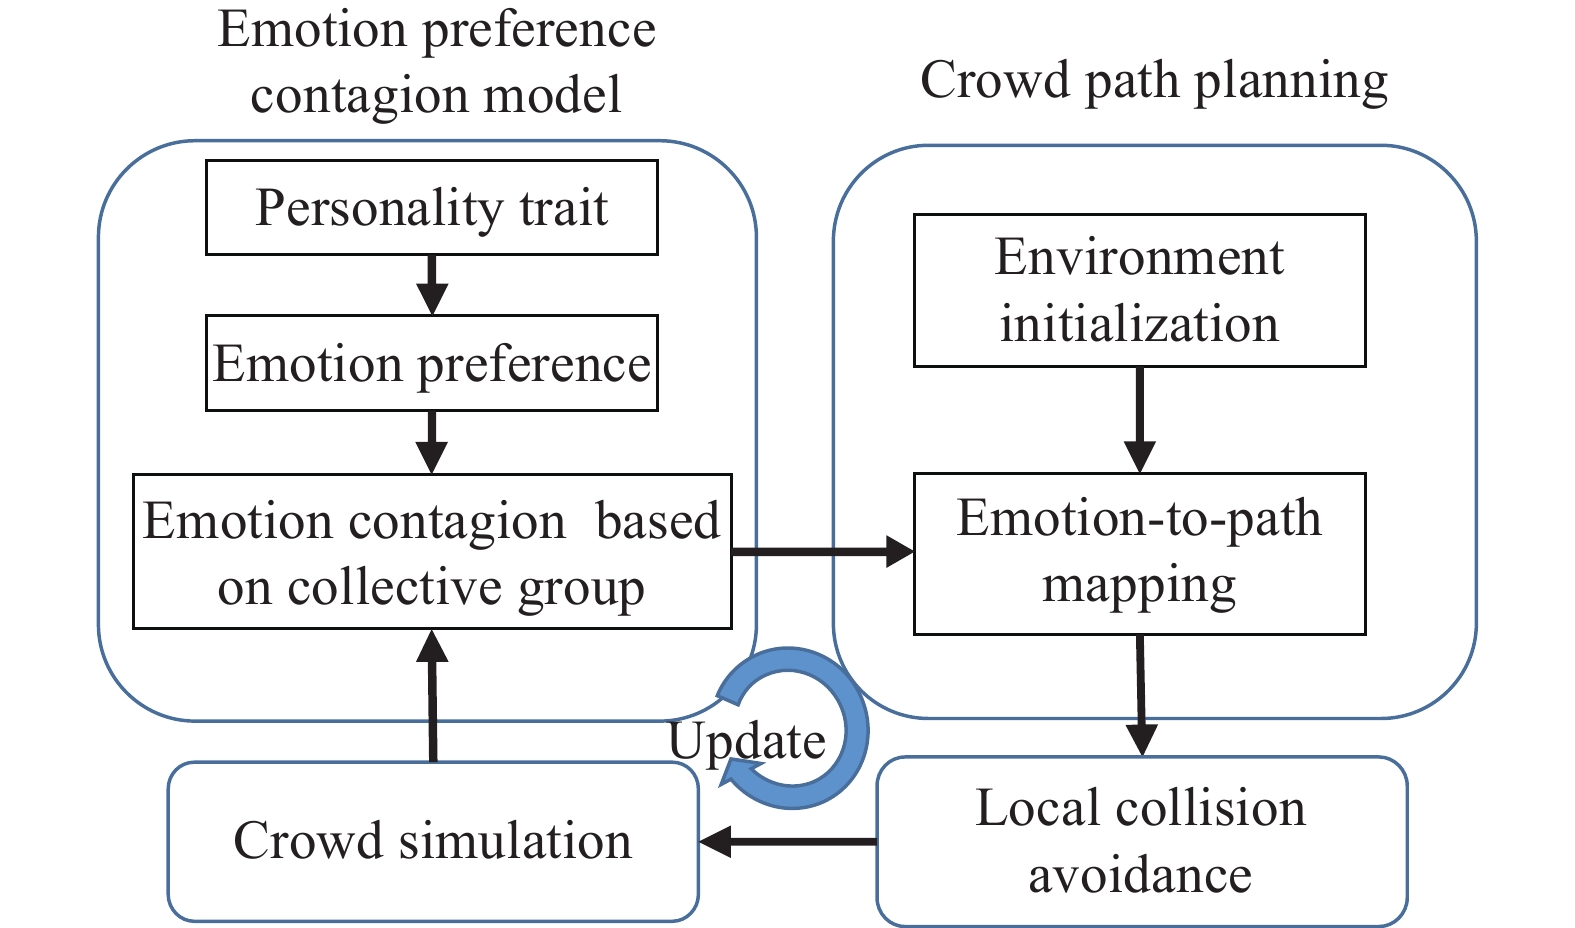
\includegraphics[width=1\linewidth]{fig/outline.jpg}
    \caption{The emotion contagion model as proposed by the source article \cite{Wu_Huang_Tian_Yan_Yu_2024}.}
    \label{fig:outline}
\end{figure}

The source article proposes generating agents with distinct values for the five OCEAN traits: openness to experience, conscientiousness, extroversion, agreeableness, and neuroticism. Based on those factors, agents are then assigned an initial distance preference ${P_d}$ and an initial velocity preference ${P_v}$. Agents have larger distance preferences if their personality factors are simple, aggressive, and fragile (corresponding to OCEAN factors: O${-}$, E${-}$, A${+}$), and agents have larger velocity preferences if their personality factors are variable, energetic, and functional (corresponding to OCEAN factors: C${-}$, E${+}$, N${+}$). If an agent has a large distance preference, its velocity preference is usually smaller, and vice versa. An agent with a larger velocity preference will seek to find less crowded paths even at the cost of the distance being longer, while those with a larger distance preference will stick to a path even as it becomes crowded. An emotion contagion mechanism further enhances the model by allowing emotional states to spread among neighboring agents, mimicking the way emotions such as stress or calm influence a group. A dampening factor regulates this contagion to ensure an agent's inherent personality traits are at least partially preserved. The model incorporates a strategy where a least expected-time objective function is used to dynamically select paths, factoring in both environmental variables and agents’ emotional states and preferences \cite{Wu_Huang_Tian_Yan_Yu_2024}.

The other aspect of the article is emotion contagion. For that purpose, the simulation requires a method to define collective clusters among the agents to determine which of them will be mutually affected. Agents are defined as being collective neighbors if they share similar motion and have a mutual goal. Information is contagious between neighboring agents in the same group and is affected by the distance between agents and the difference between emotion preferences. Additionally, agents may be affected by environmental contagious sources, such as a fire disaster \cite{Wu_Huang_Tian_Yan_Yu_2024}.  

The \textit{Simulation of crowd dynamics in pedestrian evacuation concerning panic contagion: A cellular automaton approach} article describes how panic could influence the path planning of the agent.
The authors propose a model where panic is contagious and negatively impacts the ability of an agent to find an exit \cite{Wang_2022}.
\subsection{Proposed improvements}
% Emotion memory
% We propose adding an additional \textbf{Emotion memory} parameter to the agents. The emotion memory parameter would affect the agent on a multi-run simulation where the same agents would be placed in different environments in sequence.

\subsubsection{Panic contagion}
An improvement that we propose is adding \textbf{Panic contagion} to the simulation. Each agent is assigned a panic parameter and a panic susceptibility parameter, where panic inhibits the ability of the agent to move to their goal. As the panic parameter increases, the agent's movement becomes increasingly erratic and random.

The panic susceptibility parameter, in our approach, is calculated from the OCEAN traits of the agent, as shown in Equation \ref{equ:panic}. The subscript $_0$ next to a given trait denotes the value being shifted by $0.5$ from the original expected value, so that the new expected value is equal to $0$. Openness, conscientiousness and agreeableness have negative correlation with panic susceptibility, while neuroticism has positive correlation. The distribution of panic susceptibility remains equal to the distribution of the traits: $N(0.5,0.1)$. We decided that all traits are equally important: \(w_O = w_C= w_A= w_N= \sqrt{1/4}\).

\begin{align}
    \label{equ:panic}
    panic\_susceptibility = -w_O * O_0 - w_C* C_0 - w_A* A_0 + w_N *  
    N_0 + 0.5, \\
    \text{where } w_O^2 + w_C^2 + w_A^2 + w_N^2 = 1 \nonumber
\end{align}

Each agent is assigned a current panic parameter. This parameter represents the probability that the agent will not behave according to their personality and will either freeze or move randomly. This parameter can be modified in three ways. Every agent seeks to reduce their panic to a baseline level, the return to the baseline level being dependent on their panic susceptibility parameter. The relationship is described in Equation \ref{equ:panic_decress} for every $\Delta{t}$.

\begin{equation}
    current\_panic \mathrel{-}= (0.5 + (0.01 - 0.5) \cdot panic\_susceptibility) * (current\_panic)
    \label{equ:panic_decress}
\end{equation}

There are two means by which the panic parameter of an agent may increase. Agents are susceptible to the panic of other agents in their cluster and their panic parameter value will accordingly change to match the cluster's average, with the speed of the change governed by their panic susceptibility, as described by Equation \ref{equ:panic_clustenr_inc}. 

\begin{equation}
  \begin{aligned}
    panic\_\text{\textit{diff}} = average\_cluster\_panic - current\_panic \\
    current\_panic \mathrel{+}= panic\_susceptibility * panic\_\text{\textit{diff}} * 0.05
\end{aligned}
    \label{equ:panic_clustenr_inc}
\end{equation}

An agent's current panic may also increase if they are near a panic-inducing source, which is described by Equation \ref{equ:panic_inuction}.
\begin{equation}
    \begin{aligned}
        dist = \frac{1} {|position - panic\_source\_position|} \\
        current\_panic += dist * panic\_susceptibility * 0.001
    \end{aligned}
    \label{equ:panic_inuction}
\end{equation}

\subsubsection{Clustering algorithm evaluation}
It was also be possible to explore how the \textbf{clustering algorithm} described in the article performs when compared to hierarchical clustering and Fast Label Propagation \cite{Lovre_2023}.
% generalized community detection algorithms, such as Leiden \cite{Leiden}, Walktrap \cite{Walktrap}, or (Fast) Label Propagation \cite{Lovre_2023}.

% We plan to test how the grid resolution affects the movement of agents.

\subsubsection{Enhanced navigation graph} Additional movement options have been added to the navigation graph, as described in Section \ref{res}.


\subsubsection{Corrected error}
We believe to have found \textbf{an error in the source article} with its equation: \begin{equation*}
    d_{ori}(i,j)=|arccos(vel_i)-arccos(vel_j)|
\end{equation*}
which does not appear to be a operation that can be performed on a vector, so we instead propose: \begin{equation*}
    d_{ori}(i,j)=|atan2(vel_{i_y},vel_{i_x})-atan2(vel_{j_y},vel_{j_x})|
\end{equation*}
where we obtain the correct angle ${\theta}$\ from the \textit{x}-axis \cite{wikiatan2} for each of a pair of agents and then subtract the angles to obtain the difference between their orientations.

% RESULTS
\section{Results} \label{res}
\subsubsection{Clustering}
Figure \ref{fig:enter-label} shows multiple runs of the clustering algorithm from article \cite{Wu_Huang_Tian_Yan_Yu_2024}. Even though the clusters were very different when we used a different algorithm, little to no effect was visible on the agent paths.

\begin{figure}[h!]
    \centering
    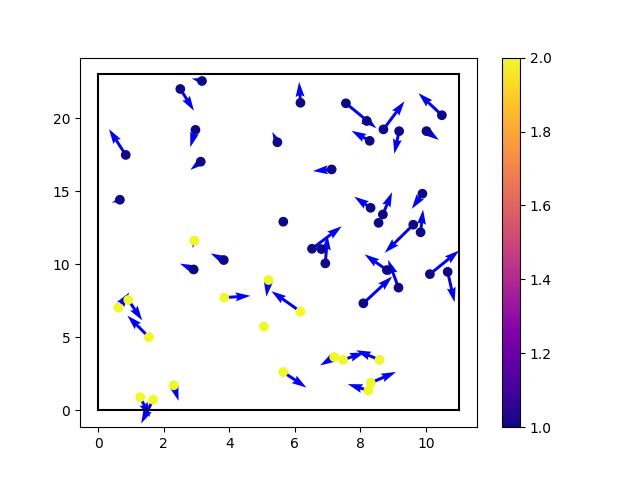
\includegraphics[width=0.3\linewidth]{fig/Figure_2.png}
    \hfill
    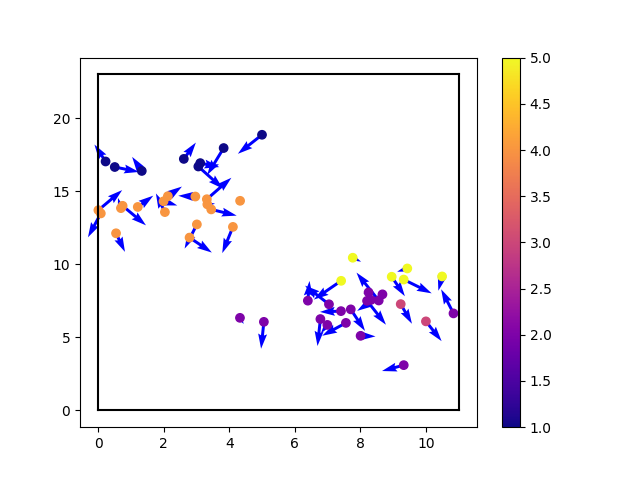
\includegraphics[width=0.3\linewidth]{fig/Figure_3.png}
    \hfill
    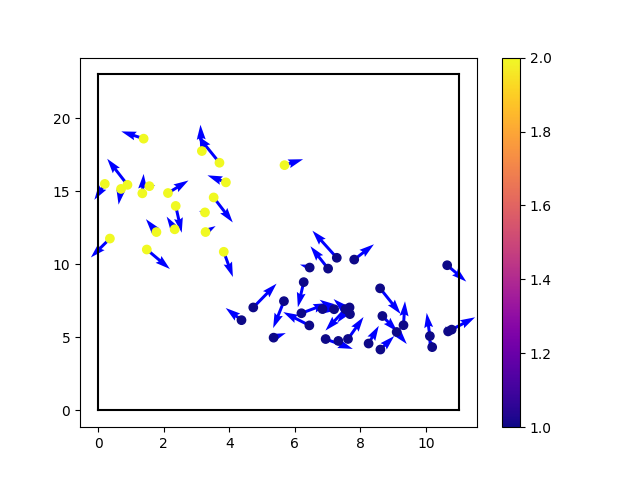
\includegraphics[width=0.3\linewidth]{fig/Figure_4.png}
    \caption{Example runs of clustering according to association with the closest neighbor with a higher degree. The leftmost sub-figure represents agents with positions initialized uniformly, while the two to the right represent agents with positions initialized with a bimodal Gaussian distribution.}
    \label{fig:enter-label}
\end{figure}

\subsubsection{Navigation graph}

For each exit we constructed a navigation graph of shortest paths. Every such graph is a tree or a forest with roots among the nodes belonging to an exit, representing shortest paths from all possible positions on the grid to one of the exits. It was constructed using Dijkstra's algorithm allowing movements to all 8 neighboring fields as well 
as to fields located two steps in one direction and one step in a perpendicular direction.
An example graph is shown in Figure \ref{fig:spgraph}.

This navigation graph would, in theory, allow for modeling the movement of agents in a more natural way than the basic left-right-up-down version of it.

\begin{figure}[h!]
    \centering
    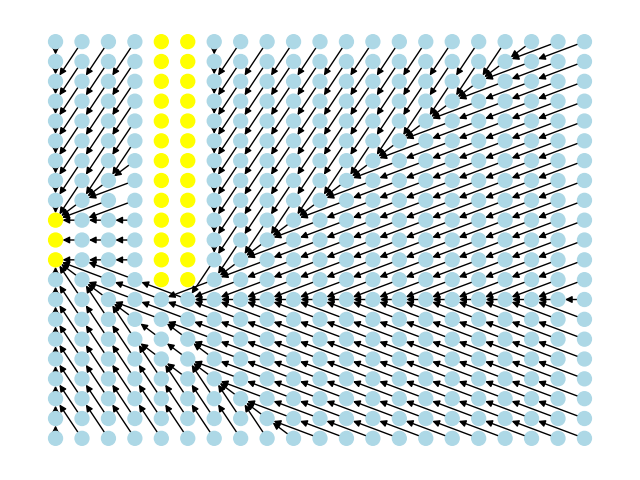
\includegraphics[width=0.5\linewidth]{fig/dijkstra.png}
    \caption{Example navigation graph for a grid of dimensions 10 times 10. Yellow nodes represent the exit of width 3 and the obstacle.}
    \label{fig:spgraph}
\end{figure}

% \begin{figure}
%     \centering
%     \includegraphics[width=0.5\linewidth]{fig/plots/obst_nopanic_oldclusters_path_plot.png}
%     \caption{Path of agents in the environment with obstacles no panic and clustering algorithm proposed by the authors of the original paper.}
%     \label{fig:obst_nopanic_oldclusters_plot_path}
% \end{figure}

% \begin{figure}
%     \centering
%     \includegraphics[width=0.5\linewidth]{fig/plots/obst_nopanic_newclusters_path_plot.png}
%     \caption{Path of agents in the environment with obstacles no panic and clustering algorithm proposed by the authors of the original paper.}
%     \label{fig:obst_nopanic_oldclusters_plot_path}
% \end{figure}

\subsubsection{Experiment}
We performed an experiment where we manually set the velocity preference of a single agent to a significantly higher value than the other agents. The results can be seen in Figure \ref{fig:outlier}.
\begin{figure}[htb]
    \centering
    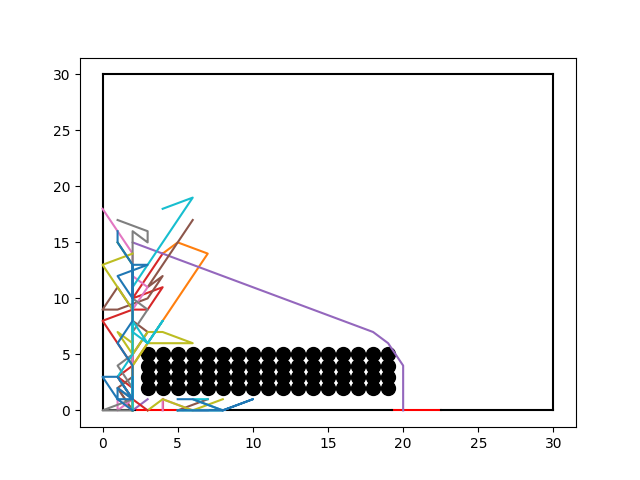
\includegraphics[width=0.5\linewidth]{fig/path_plot_single_outlier.png}
    \caption{Paths of the agents in the case of a single agent assigned a very strong velocity preference, forcing them to choose the farther exit. The black dots represent an arbitrary obstacle.}
    \label{fig:outlier}
\end{figure}

\subsubsection{Panic}
We discovered that the panic parameter has great influence on the paths, as shown in Figure \ref{fig:panic}.

\begin{figure}[h!]
    \centering
    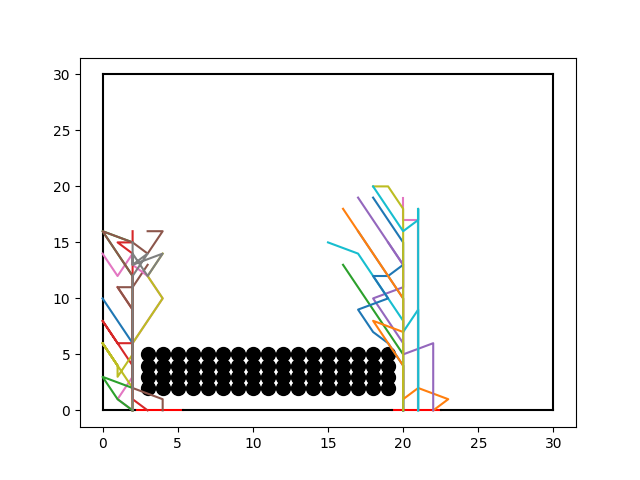
\includegraphics[width=0.45\linewidth]{fig/path_plot_nopanic.png}
    \hfill
    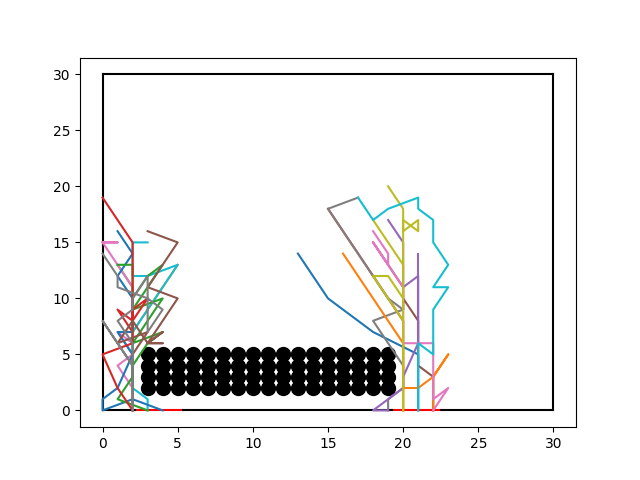
\includegraphics[width=0.45\linewidth]{fig/path_plot_panic.png}
    \caption{Example runs without a source of panic (left) and with a source of panic (right) included. The more erratic movement as a result of the panic is clearly seen in the right part of the figure.}
    \label{fig:panic}
\end{figure}

\subsubsection{Testing of hierarchical clustering algorithm}

We tested the hierarchical clustering algorithm and found that the results are no different than with the clustering algorithm proposed by the source article.

\begin{figure}[h!]
    \centering
    \includegraphics[width=0.45\linewidth]{fig/obst_nopanic_newclusters_path_plot.png}
\hfill
    \includegraphics[width=0.45\linewidth]{fig/obst_nopanic_oldclusters_path_plot.png}
    \caption{The left image represents the paths of the agents that were clustered using hierarchical clustering and the image on the right represents the paths of agents based off the clustering algorithm proposed by the source article.}
    \label{fig:enter-label}
\end{figure}

% DISCUSSION
\section{Discussion}
We have implemented a simulation workflow where we can define the environment in the text format and then run the simulations. We tried out three different clustering algorithms, but the change of clustering algorithm appears to have no visible influence on the result. The introduction of panic parameter was a fruitful decision, as panic like behavior can be seen in the paths of agents.

Many aspects of the implementation had to be reinvented, as the authors of article \cite{Wu_Huang_Tian_Yan_Yu_2024} at some points did not elaborate on their solutions. One such instance was with the implementation of the navigation graph generation, as for small environment sizes in the range of $100\times 100$ tiles were reasonably fast, but larger environments were not feasible as the time to construct the graph was excessive. To allow for greater precision of agent movement, it would be preferable to optimize the navigation graph generation or at least cache it for repeated use.

Future work could explore alternatives for the navigation graph that would allow for the agent positions to be points instead of real numbers. Additionally, the agent paths could be curves parametrized by continuous time parameters, which would allow for continuous time instead of discrete time steps.

\acknow{\textbf{AS} worked on the code (environment representation, agent movement) and on the report, \textbf{TZ} worked on the report and its editing as well as proofreading, and oversaw project management, and \textbf{ELG} worked on the code (contagion, navigation graph, clustering, visualization) and on the report.}
\showacknow % Display the acknowledgments section

% \pnasbreak splits and balances the columns before the references.
% If you see unexpected formatting errors, try commenting out this line
% as it can run into problems with floats and footnotes on the final page.
%\pnasbreak

\begin{multicols}{2}
\section*{\bibname}
% Bibliography
\bibliography{./bib/bibliography}
\end{multicols}

\end{document}